%
% Chapter 7
%
\chapter{Development of a Formal Testing Procedure}
\section{Initial considerations}
The new procedure was desgined as a direct response to the previous one. Based on complaints and difficulties from all who had to use the setup, we compiled a list of the biggest concerns and focused the procedure design around them. These included:
\begin{itemize}
	\item Manually changing input/output channels was slow and introduced too many steps
	\item Input \& output were connected through a flimsy probe clip
	\item No way to separate amp power rails
	\item No indication if the amps were receiving sufficient power
	\item No data collection for comparison between cards
	\item No standards or documentation for gain/offset potentiometer tweaks
\end{itemize}
\section{Design Choices}
The first readily apparent issue lay in the fact that there was a great deal of manual setup being performed by testers which was not ideal for long-term or large-scale testing. Amp cards were delivered in relatively small batches and had to be reworked and tested as they came. Having to search for a procedure that was hard to understand was not a good solution. I opted to use Python drivers communicating over the two serial specifications (USB serial and VX11 over Ethernet) to automate the input generation and output measurement. By having direct software access to the wave being generated and the data collection, users were in control of a closed loop from beginning to end. The remainder of the issues remained in the lack of hardware support for testing. Input and output locations were unclear and pin placement was only known to those who created the boards, unless testers wanted to open the PCB files and check themselves. By designing a pair of new PCBs to solve this issue, the test station had a clear set of instructions and devices to measure and capture data as was needed.

\section{Software Control}
Controlling the instruments available in our lab took a bit of research. While other group members had used some of the automation tools before, this was one of the first fully scripted hardware test setups in the lab. The communication protocols and code libraries required are explored below.
\subsection{pySerial Overview}
PySerial is a simple Python library to build and push serial commands over a variety of protocols. This library allows programmers to script serial access and build their own commands to be used for any device they require. For this application, I needed to build commands for a function generator. Other members of the group had previously automated this device and were able to provide documentation on the serial commands necessary. The benefit of a simple serial protocol was that it required no proprietary software and could be modified or extended for other devices. Initiating communication with a serial device is simple with pySerial as the programmer can simply can all serial ports and view device properties. In this specific application the serial device was the only one connected to the host computer, which allowed the device detection to be quite straightforward:\par
\begin{lstlisting}
	ports = list(serial.tools.list_ports.comports())
	for port, desc, hwid in sorted(ports):
		print("{}: {} [{}]".format(port, desc, hwid))
	for p in ports:
		print("USB Serial: {}".format(p.description))
		if "USB-SERIAL" in p.description:
				print("Found the FeelTech AWG")
				awg = feeltech_awg.FeelTechAWG(p[0])
	assert awg is not None, "No AWG device found"
\end{lstlisting}
To understand the process of communicating with this device I traced example commands to their lowest levels. To command the device to do anything, requests first had to be packaged into a recognizable prefix. To generate a prefix, parameters must be packaged in a particular order: \par
\begin{lstlisting}
	assert rw in range(2), "R/W value for prefix must be 0 (read) or 1 (write)"
	prefix_rw = "W" if rw == 1 else "R"
	assert channel in (1, 2), "Invalid channel, must be set to 1 (main) or 2 (auxilary)."
	prefix_channel = "M" if channel == 1 else "F"
	valid_modifiers = ("W", "F", "A", "O", "D", "P", "N")
	assert modifier in valid_modifiers, "Invalid cmd modifier (%s), must be in %s"%(modifier, valid_modifiers)
	return prefix_rw + prefix_channel + modifier
\end{lstlisting}
This command prefix is then concatenated with a desired parameter based on the function being controlled. Turning on an output channel, for example, takes in an output flag and attaches it to the command prefix:
\begin{lstlisting}
	"""
	output:  int -> 0 to turn channel off, 1 to turn channel on
	"""
	cmd = _generate_cmd_prefix(1, channel, "N") + str(output)
\end{lstlisting}
The command is now ready to be sent to the device. Using pySerial functions for read/write operations, the code is simple:
\begin{lstlisting}
	self.device.flushInput()
	self.device.write((cmd_str + "\n").encode())
	self.device.flush()
\end{lstlisting}
The straightforward nature of serial communications made this easy to debug and test. The function generator only needed to perform a few tasks (turn channels on/off, set waveform parameters) the scope of my research into its functionality was limited. I believe, however, that this establishes a good base for future testing development. Many other instruments use specifications such as VISA which may be a better choice in the future.

\subsection{VXI11 Overview}
The VXI11 Communication Protocol is an architecture based on the VMEbus architecture meant for electronic communication. VXI11 in particular was built as an instrument communication spec \cite{vxi}. VXI11 requires three channels and operates over Ethernet. An abstract view of the communication network is attached below.
\begin{figure}
	\centering
	\includegraphics*[width=0.8\textwidth]{vxi11}
	\caption{VXI Core, Abort and Interrupt channels \cite{vxi}}
\end{figure}
VXI11 Python libraries are available and make VXI communication simple. Similarly to serial, commands must be constructed by the programmer and packaged into strings sent over the VXI bus. For example, writing to the device makes a device-level system call to write the input data to a predetermined location. From the programmer's point of view, one only has to use the high-level functions to facilitate communication. There are, for example, functions for read(), write(), and ask(), which performs a write and then read. These functions are grouped and abstracted for use with this specific instrument. If, for example, the programmer wants to ask the device what a selected channel's probe ratio is, the code is as follows:
\begin{lstlisting}
	def get_probe_ratio(self, channel):
		"""
		Returns the probe ratio for a specific channel
		"""
		channel = self._interpret_channel(channel)
		return float(self.query(':{0}:PROBe?'.format(channel)))
\end{lstlisting}
The string being pushed in the query function is a device-specific string that is outlined by the manufacturer \cite{rigol}. Using the listed commands and an ethernet connection, the VXI11 bus will automatically detect when a valid device is connected to the local network through Ethernet. The IP address of the device is specified upon initialization and needs to be checked before running tests.

\section{Input Stage}
The input stage of the amp testing procedure was the first to be targeted. Directing input to the amp card should be a simple task for the user. Since all four channels are used in parallel on the system, they can be connected to a unified signal source and displayed together on the oscilloscope for data collection. Using a mix of hardware and software support I developed an input procedure for the new test.
\subsection{Function Generation}
To implement a Python layer for the function generator I opted to use a FeelTech FY6900 Arbitrary Waveform Generator.
\begin{figure}[!htb]
	\centering
	\includegraphics*[]{awg}
	\caption{FeelTech FY6900}
\end{figure}
This was a relatively cheap function generator that fulfilled the tasks we needed to accomplish. With up to 60MHz sine wave output, this device was more than enough to test the capabilities of the amplifiers. The DAC input the amps were designed to process were at frequencies far below this. For the first versions of the test I opted to use the original function generator settings until more could be determined about the input parameters. The code was simple and based on the previously listed libraries \& protocols:
\begin{lstlisting}
	awg.set_on_off(1, 0)
	awg.set_on_off(2, 0)

	awg.set_waveform(1, 1)
	awg.set_frequency(1, 1000000)
	awg.set_amplitude(1, x[i])
	awg.set_offset(1, 0.318)
	awg.set_phase(1, 0)

	# Turn channel 1 on
	awg.set_on_off(1, 1)
\end{lstlisting}
For the automated test to save time, it was set to loop four times to collect plot data from the oscilloscope for all four amplifier output channels. In order for this automatic switching to work, hardware had to be designed to accept the signal and distribute it accordingly.
\subsection{Bottom (Input) PCB}
Major flaws in the original test setup included the lack of any shielded cable to transfer the input signal and the tester having to manually clip the input to each amp channel. Although we were not necessarily testing for strict signal integrity, it is better practice to use standard connectors for input rather than probe clips. Since the FeelTech generator used a BNC connector it was easiest to match this on the input card. BNC connectors are shielded coaxial connectors capable of reliably passing signals under 4GHz and less than 500V \cite{bncbook}. \par
Separating the amplifier's input lines was a useless step that only served to complicate the process. To solve this I had to examine the amp's PCB layout to find the relevant pins. The DAC inputs were differential pairs identified within the layout below:
\begin{figure}[!htb]
	\centering
	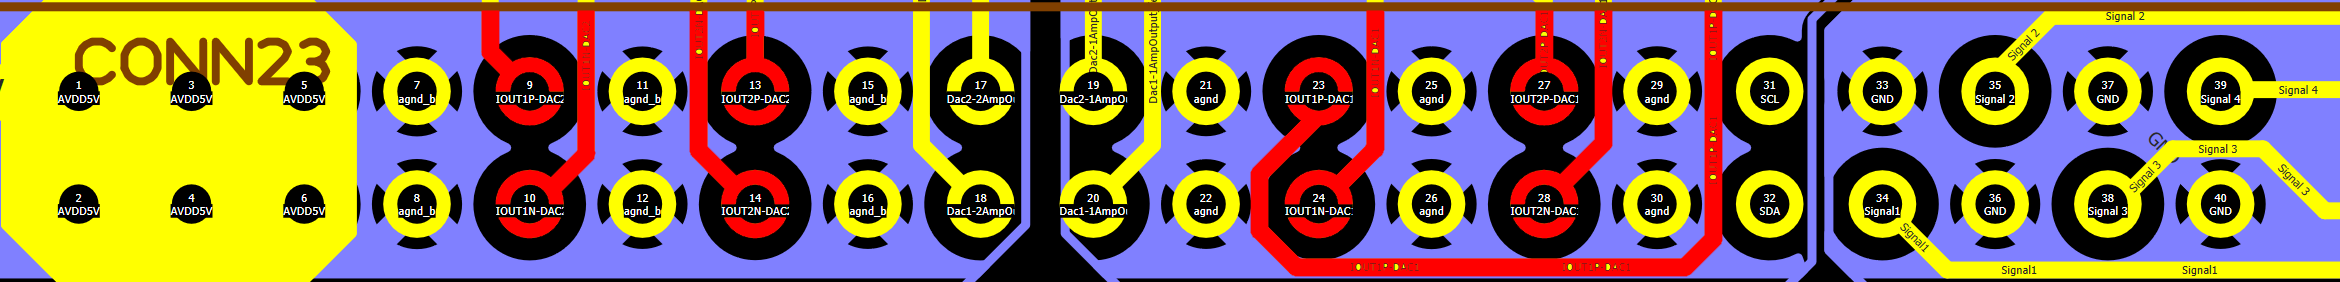
\includegraphics[width=\textwidth]{amp_input_pins}
	\caption{Differential input pins on the Amp PCB}
\end{figure}
The input side of the board was fairly simple to draw and lay out. One of the amp's purposes was to turn the DAC's differential output into a single-ended output. To accomplish this, the amp card terminated the N-terminals of all incoming DAC signals through a 49 ohm resistor.
\begin{figure}[!htb]
	\centering
	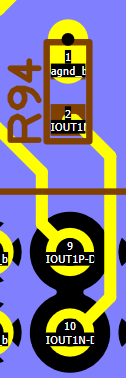
\includegraphics{amp_n_p}
	\caption{Terminating resistor for the N-terminal of the DAC output.}
\end{figure}
Grounding the differential input was an acceptable decision for the test setup. Only the P-lines of the signal would be processed by the circuit at all, so they were routed together and joined to a single BNC input in the test board.
\begin{figure}[!htb]
	\centering
	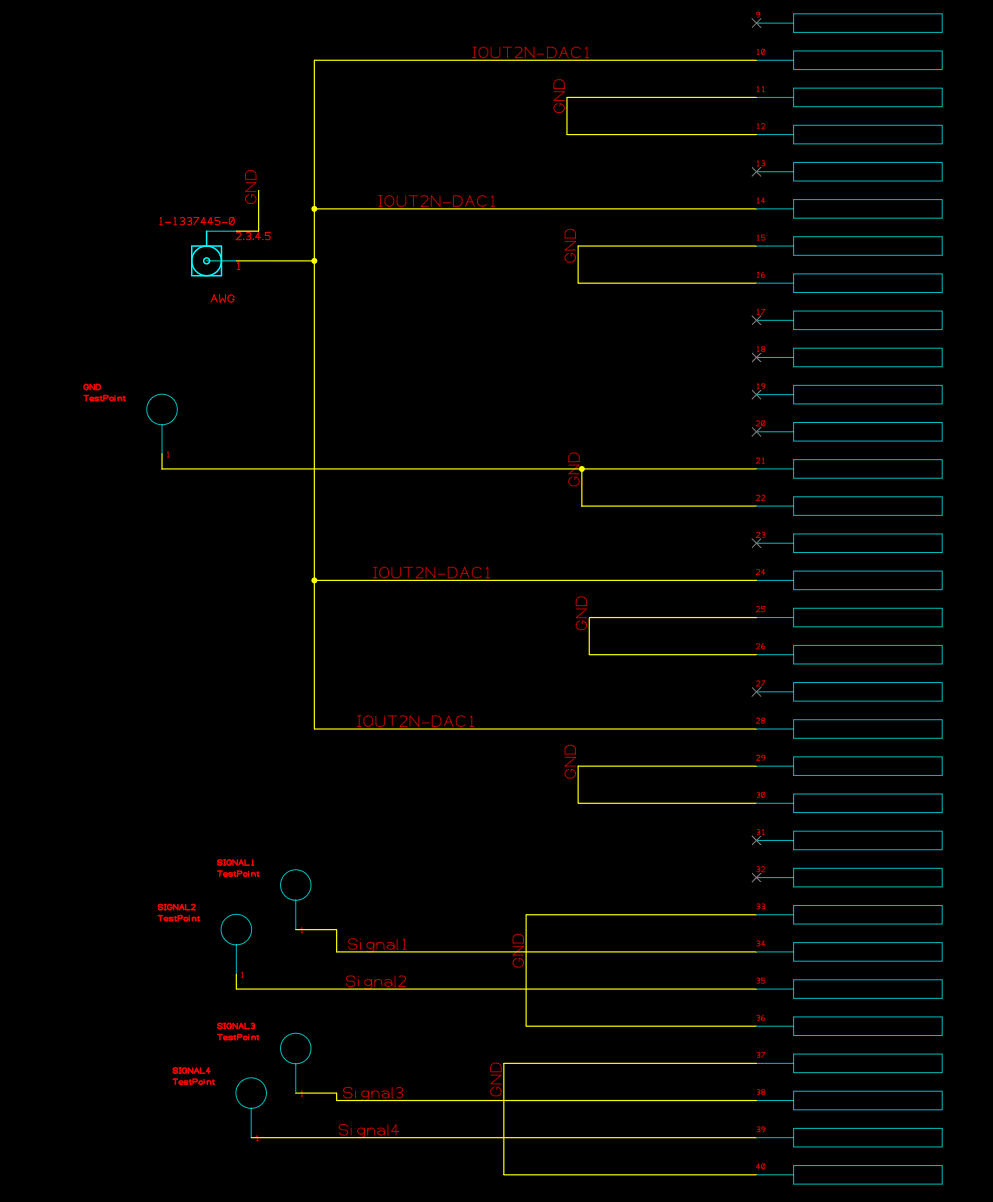
\includegraphics[width=\textwidth]{amp_bottom_schematic.png}
	\caption{Input Test board schematic for joining P-inputs and grounding N-inputs}
\end{figure}
The layout followed shortly and included a ground plane to maximize signal integrity. With such a limited number of relevant pins on the input side of the amp card, designing the test board was not an issue. \par
\begin{figure}[!htb]
	\centering
	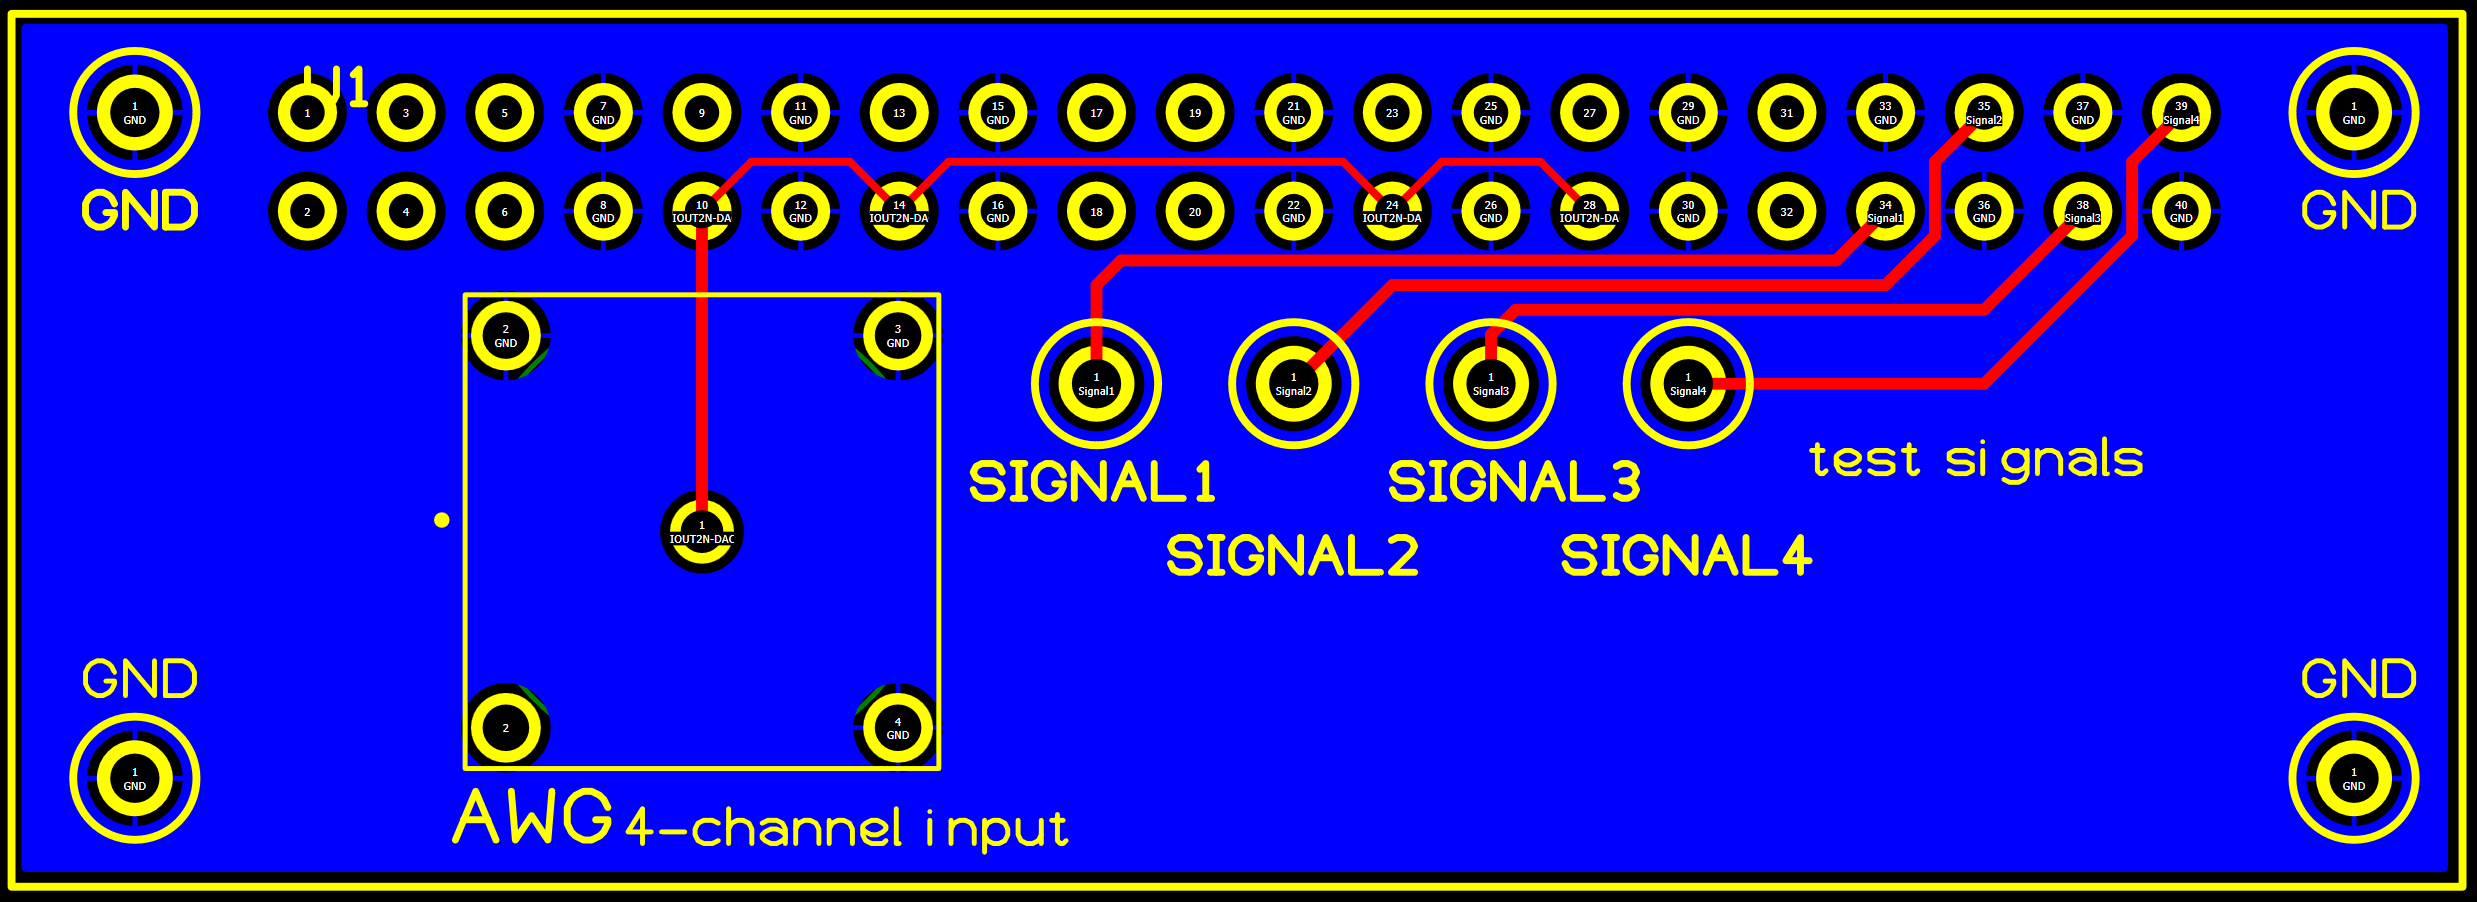
\includegraphics[width=\textwidth]{amp_bottom_layout.png}
	\caption{Input Test board layout}
\end{figure}
\subsection{Input Conclusion}
This section of the test setup resulted in a far simpler procedure. Having to only connect one output through a stable connection and clearly labeled board eliminated all possible confusion for testers. INSERT PICTURE OF BOARD HERE

\section{Output Stage}
The output of the amp card required the testers to be able to view all output channels at once as well as collect and plot the oscilloscope's data. This once again required a mix of software and hardware tools to accomplish.